\documentclass[conference]{IEEEtran}

\usepackage{cite}
\usepackage{amsmath,amssymb,amsfonts}
\usepackage{graphicx}
\usepackage{booktabs}
\usepackage{url}

% Keep floats tight to their referencing sections in two-column IEEEtran layout.
\renewcommand{\topfraction}{0.90}
\renewcommand{\bottomfraction}{0.80}
\renewcommand{\textfraction}{0.07}
\renewcommand{\floatpagefraction}{0.65}
\renewcommand{\dbltopfraction}{0.88}
\renewcommand{\dblfloatpagefraction}{0.65}
\setcounter{topnumber}{4}
\setcounter{bottomnumber}{3}
\setcounter{totalnumber}{6}
\setcounter{dbltopnumber}{2}
\setlength{\textfloatsep}{7pt plus 2pt minus 2pt}
\setlength{\dbltextfloatsep}{8pt plus 2pt minus 2pt}
\setlength{\intextsep}{7pt plus 2pt minus 2pt}

\begin{document}

\title{Hyperspherical Metric Learning and Failure Analysis of Confidence and Global-SVDD Boundaries for Open-Set Underwater Sonar Recognition}

\author{
\IEEEauthorblockN{Muhammad Haroon}
\IEEEauthorblockA{Department of Computer Science\\
Bahria University\\
Islamabad, Pakistan}
\and
\IEEEauthorblockN{Muhammad Khizar Hayat Cheema}
\IEEEauthorblockA{Department of Computer Science\\
Bahria University\\
Islamabad, Pakistan}
\and
\IEEEauthorblockN{Arif Ur Rahman}
\IEEEauthorblockA{Department of Computer Science\\
Bahria University\\
Islamabad, Pakistan}
}
% Institutional author emails may be added inside each IEEEauthorblockA block per CFP requirements.

\maketitle

\begin{abstract}
Closed-set classifiers trained on underwater forward-looking sonar (FLS) imagery frequently assign high confidence to unmodeled subsea debris, risking collisions and misidentifications during autonomous underwater vehicle deployment. We evaluate open-set recognition on the 2,364-image Marine Debris Forward-Looking Sonar (MD-FLS) water-tank benchmark under a six-known / four-unknown partition containing morphologically similar container classes. Comparing post-hoc Maximum Softmax Probability (MSP) thresholding, three 2048-D Support Vector Data Description (SVDD) boundaries, and end-to-end hyperspherical Deep Metric Learning (DML) on the 128-D unit sphere exposes two geometric failure modes. First, softmax exponentiation over unbounded logit sectors pushes unknown confidences close to unity; Youden calibration selects 0.9980 and limits MSP to 0.9069 AUROC and 0.7747 Average Precision (AP). Second, enclosing cross-entropy features inside a single Global Centroid SVDD sphere collapses to 0.2371 AUROC because known classes sit on outer high-norm radial lobes while unknown objects project near the global mean. Class-conditional Nearest Centroid SVDD recovers to 0.9175 AUROC (0.8568 AP). End-to-end EmbeddingNet trained with cosine Triplet Margin Loss wins all five metrics at 0.9603 AUROC, 0.9235 AP, 0.9013 Unknown Detection Rate, 0.0987 False Positive Rate, and 0.9077 True Positive Rate, with 100.0\% closed-set nearest-centroid known accuracy.
\end{abstract}

\begin{IEEEkeywords}
Forward-looking sonar, open-set recognition, deep metric learning, support vector data description, underwater debris.
\end{IEEEkeywords}

\section{Introduction}
\label{sec:intro}

Autonomous underwater vehicles (AUVs) operating in dark or turbid coastal waters depend on forward-looking sonar (FLS) to detect and classify submerged debris~\cite{valdenegro_2016_oceans,valdenegro_2017_oceans}. Convolutional neural networks (CNNs) classify cataloged acoustic targets accurately~\cite{williams_2016_icpr,valdenegro_2025_datasets}, yet ocean deployment regularly introduces uncataloged rigging, discarded containers, and seabed clutter. Closed-set softmax classifiers map every acoustic return onto fixed training labels and often emit saturated confidence on unseen objects~\cite{scheirer_2013_osr,bendale_2016_openmax}.

Separating known and unknown sonar objects is difficult for three physical and geometric reasons. Acoustic crops lack chromatic cues, carry multiplicative speckle noise with strong cross-class brightness shifts, and project three-dimensional objects onto two-dimensional range-azimuth planes. Distinct objects can therefore produce overlapping bright echoes and acoustic shadows, causing near out-of-distribution (near-OOD) ambiguity~\cite{vaze_2022_osr}. Recent sonar open-set work investigates logit calibration and Extreme Value Theory (EVT) under class imbalance~\cite{jiao_2024_sonar_osr,li_2026_copenmax}. Two geometric questions remain unmeasured on this benchmark: why single-center SVDD collapses on cross-entropy sonar features~\cite{tax_2004_svdd,chong_2020_ijcnn}, and how unit-hypersphere metric bounds~\cite{schroff_2015_facenet,musgrave_2020_pml} compare against softmax confidence compression.

We compare Maximum Softmax Probability (MSP) thresholding~\cite{hendrycks_2017_msp}, three 2048-D Global Average Pooling (GAP) SVDD formulations~\cite{scholkopf_2001_ocsvm,tax_2004_svdd}, and end-to-end hyperspherical Deep Metric Learning (DML) on the MD-FLS water-tank dataset~\cite{singh_2021_iccvw,valdenegro_2025_datasets} (Fig.~\ref{fig:overview}). All methods share deterministic median and CLAHE preprocessing~\cite{zuiderveld_1994_clahe}, identical dataset splits, and Youden operating-point selection~\cite{youden_1950_index}.

This work makes three contributions:
\begin{enumerate}
    \item A deterministic, leak-free near-OOD FLS benchmark on 2,364 MD-FLS water-tank images (1,233 train, 262 validation, 869 test) withholding \texttt{chain}, \texttt{valve}, \texttt{shampoo-bottle}, and \texttt{standing-bottle} alongside six known classes including \texttt{bottle}.
    \item Empirical diagnosis of two post-hoc failure modes on sonar representations: MSP score compression at $\tau^* = 0.9980$ (0.7747 AP) and Global Centroid SVDD collapse (0.2371 AUROC), rescued to 0.9175 AUROC by Nearest Class Centroids.
    \item Evidence that end-to-end hyperspherical metric learning (\texttt{EmbeddingNet} on $\mathbb{S}^{127}$ under cosine Triplet Margin Loss and online hard mining) leads all five OSR metrics (0.9603 AUROC, 0.9235 AP, 0.9013 UDR, 0.0987 FPR, 0.9077 TPR), keeps 100.0\% closed-set known accuracy, and lifts rejection of the hardest unknown class (\texttt{chain}) to 80.53\%.
\end{enumerate}

\begin{figure*}[!t]
    \centering
    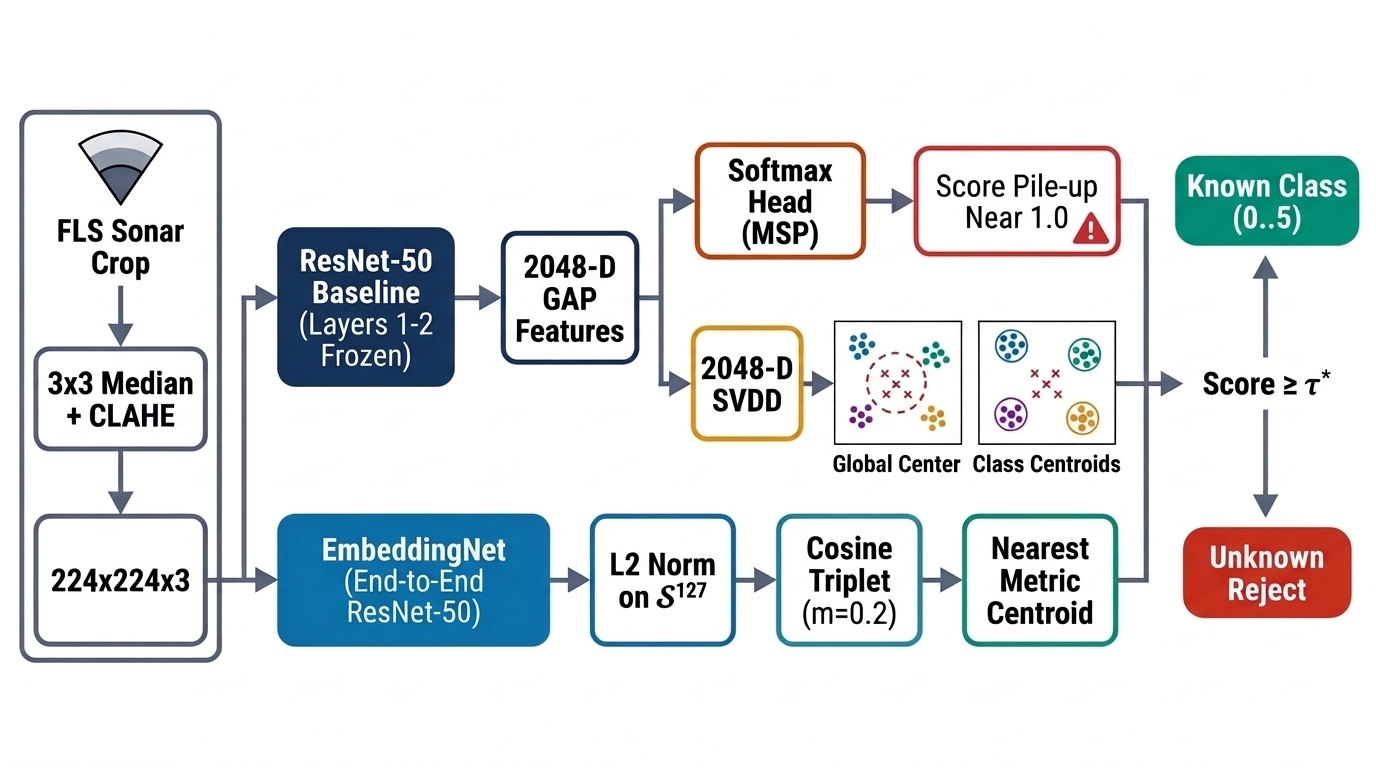
\includegraphics[width=0.72\textwidth]{figures/fig_overview.png}
    \caption{Open-set sonar recognition architecture. Identical $3\times 3$ median-filtered and CLAHE-normalized $224\times 224\times 3$ crops feed two ResNet-50 branches: the closed-set baseline (driving MSP and three 2048-D GAP SVDD boundaries) and \texttt{EmbeddingNet} trained end-to-end onto $\mathbb{S}^{127}$ under cosine Triplet Margin Loss ($m=0.2$) for nearest-centroid scoring.}
    \label{fig:overview}
\end{figure*}

\section{Related Work}
\label{sec:related}

\subsection{Deep Learning for Underwater Sonar Imagery}
CNN models introduced for underwater acoustic perception~\cite{valdenegro_2016_oceans,valdenegro_2017_oceans,williams_2016_icpr} showed that learned filters handle speckle and aspect shifts better than handcrafted descriptors on FLS and synthetic aperture sonar data. Singh and Valdenegro-Toro~\cite{singh_2021_iccvw} compiled debris scenes from a 3.0~MHz Sound Metrics ARIS Explorer 3000 sonar, later expanded into the multi-site MD-FLS benchmarks~\cite{valdenegro_2025_datasets}. Because those benchmarks address closed-set recognition and segmentation, open-set near-OOD failure modes on MD-FLS remain underexamined.

\subsection{Open-Set Recognition and Sonar Calibration}
Scheirer et al.~\cite{scheirer_2013_osr} defined open-set recognition as balancing empirical risk against open space risk outside known training support. Bendale and Boult~\cite{bendale_2016_openmax} showed that deep softmax heads assign high probabilities to unfamiliar inputs and introduced EVT-based OpenMax, while Hendrycks and Gimpel~\cite{hendrycks_2017_msp} established MSP thresholding as a standard baseline; Geng et al.~\cite{geng_2021_survey} surveyed subsequent formulations. Vaze et al.~\cite{vaze_2022_osr} noted that stronger closed-set accuracy improves OSR yet leaves semantic near-OOD shifts difficult. In sonar imagery, Jiao et al.~\cite{jiao_2024_sonar_osr} and Li et al.~\cite{li_2026_copenmax} studied long-tail open-set recognition using logit and Class-Balanced OpenMax calibration on separate datasets. We examine the complementary question of how post-hoc softmax and SVDD feature boundaries fail geometrically on MD-FLS relative to cosine triplet metric embeddings.

\subsection{One-Class Boundaries and Hyperspherical Metric Learning}
One-Class SVM~\cite{scholkopf_2001_ocsvm} and Support Vector Data Description (SVDD)~\cite{tax_2004_svdd} learn boundary support for normal data without unseen training examples. On deep representations, however, single-center hypersphere formulations can suffer collapse or fail when supervised features split across isolated class clusters~\cite{chong_2020_ijcnn}. Deep metric learning via triplet losses~\cite{hoffer_2015_triplet} and online hard mining on L2-normalized unit hyperspheres~\cite{schroff_2015_facenet,musgrave_2020_pml} restricts embeddings to $\mathbb{S}^{d-1}$, tying Euclidean proximity directly to angular margin separation.

\section{Methodology}
\label{sec:method}

Fig.~\ref{fig:overview} depicts the evaluated OSR pipeline. Preprocessed FLS crops feed two parallel backbone paths: a fine-tuned closed-set ResNet-50~\cite{he_2016_resnet} evaluated via MSP~\cite{hendrycks_2017_msp} and 2048-D GAP SVDD boundaries~\cite{tax_2004_svdd}, and an end-to-end \texttt{EmbeddingNet} projecting onto the 128-D unit hypersphere $\mathbb{S}^{127}$ under cosine Triplet Margin Loss~\cite{schroff_2015_facenet,musgrave_2020_pml}.

\subsection{Dataset Partitioning and Near-OOD Protocol}
\label{sec:dataset}

All experiments use the \texttt{watertank-cropped} subset of MD-FLS~\cite{singh_2021_iccvw,valdenegro_2025_datasets}, comprising 2,364 valid 4-channel RGBA patches across 10 object classes (zero corrupted images). Patch dimensions vary with target geometry, from compact objects (\texttt{drink-carton} mode $50\times 52$~px) to elongated debris (\texttt{shampoo-bottle} mode $251\times 69$~px, \texttt{standing-bottle} mode $176\times 48$~px).

We partition the 10 classes into 6 known classes ($K=6$, 1,766 images) and 4 withheld unknown classes ($U=4$, 598 images, label $-1$) reserved strictly for testing. Including \texttt{shampoo-bottle} and \texttt{standing-bottle} as unseen targets alongside trained \texttt{bottle} samples establishes a near-OOD morphological twin test~\cite{vaze_2022_osr}. Within each known class, sorted filenames are shuffled with seed $42$ and split into $70\%$ training (1,233 images), $15\%$ validation (262 images), and remaining test samples (271 images). Set-intersection checks confirm zero path overlap. Together with 598 unknown samples, the open-set test set contains 869 images (Table~\ref{tab:dataset}).

\begin{table}[!htbp]
\centering
\caption{MD-FLS Water-Tank Partition, Acoustic Profile, and Weights ($\text{Seed}=42$)}
\label{tab:dataset}
\scriptsize
\setlength{\tabcolsep}{2.2pt}
\begin{tabular}{@{}lccccccc@{}}
\toprule
Class & Role & Train & Val & Test & Mode ($W{\times}H$) & SNR & $w_k$ \\
\midrule
\texttt{bottle}          & Known (0)   & 314 & 67 & 68  & $79\times 97$   & 2.69 & 0.6545 \\
\texttt{can}             & Known (1)   & 256 & 55 & 56  & $68\times 80$   & 3.13 & 0.8027 \\
\texttt{tire}            & Known (2)   & 231 & 49 & 51  & $85\times 88$   & 2.15 & 0.8896 \\
\texttt{drink-carton}    & Known (3)   & 244 & 52 & 53  & $50\times 52$   & 2.45 & 0.8422 \\
\texttt{hook}            & Known (4)   & 93  & 19 & 21  & $115\times 81$  & 2.62 & 2.2097 \\
\texttt{propeller}       & Known (5)   & 95  & 20 & 22  & $131\times 128$ & 3.67 & 2.1632 \\
\midrule
\texttt{chain}           & Unk. ($-1$) & 0   & 0  & 226 & $63\times 61$   & 3.05 & -- \\
\texttt{valve}           & Unk. ($-1$) & 0   & 0  & 208 & $91\times 102$  & 1.98 & -- \\
\texttt{shampoo-bottle}  & Unk. ($-1$) & 0   & 0  & 99  & $251\times 69$  & 2.79 & -- \\
\texttt{standing-bottle} & Unk. ($-1$) & 0   & 0  & 65  & $176\times 48$  & 3.01 & -- \\
\midrule
Total                    & 6K / 4U     & 1,233 & 262 & 869 & --            & --   & -- \\
\bottomrule
\end{tabular}
\end{table}

\subsection{Sonar Preprocessing and Class-Balanced Augmentation}
\label{sec:preproc}

Mean grayscale intensity over the first 20 samples per class spans $75.92$ (\texttt{valve}) and $76.91$ (\texttt{tire}) up to $120.40$ (\texttt{chain}). Our deterministic preprocessing function (\texttt{preprocess\_sonar}) drops the alpha channel via RGBA-to-RGB conversion, converts to grayscale, applies a $3\times 3$ median filter to attenuate acoustic speckle spikes, and equalizes local contrast via Contrast Limited Adaptive Histogram Equalization (CLAHE)~\cite{zuiderveld_1994_clahe} (\texttt{clipLimit} $2.0$, $8\times 8$ tiles). Outputs are replicated across three channels (Fig.~\ref{fig:preproc}), resized to $224\times 224$, and normalized with ImageNet statistics.

Training batches of size $32$ apply horizontal flips ($p=0.5$), vertical flips ($p=0.3$), $\pm 15^\circ$ rotations, and brightness/contrast jitter ($0.2$). Validation and test passes disable stochastic augmentation. To balance majority and minority known categories ($314$ \texttt{bottle} vs. $93$ \texttt{hook}), cross-entropy applies inverse-frequency weights $w_k = N_{\text{train}} / (K N_k)$ from $0.6545$ (\texttt{bottle}) to $2.2097$ (\texttt{hook}).

\begin{figure}[!htbp]
    \centering
    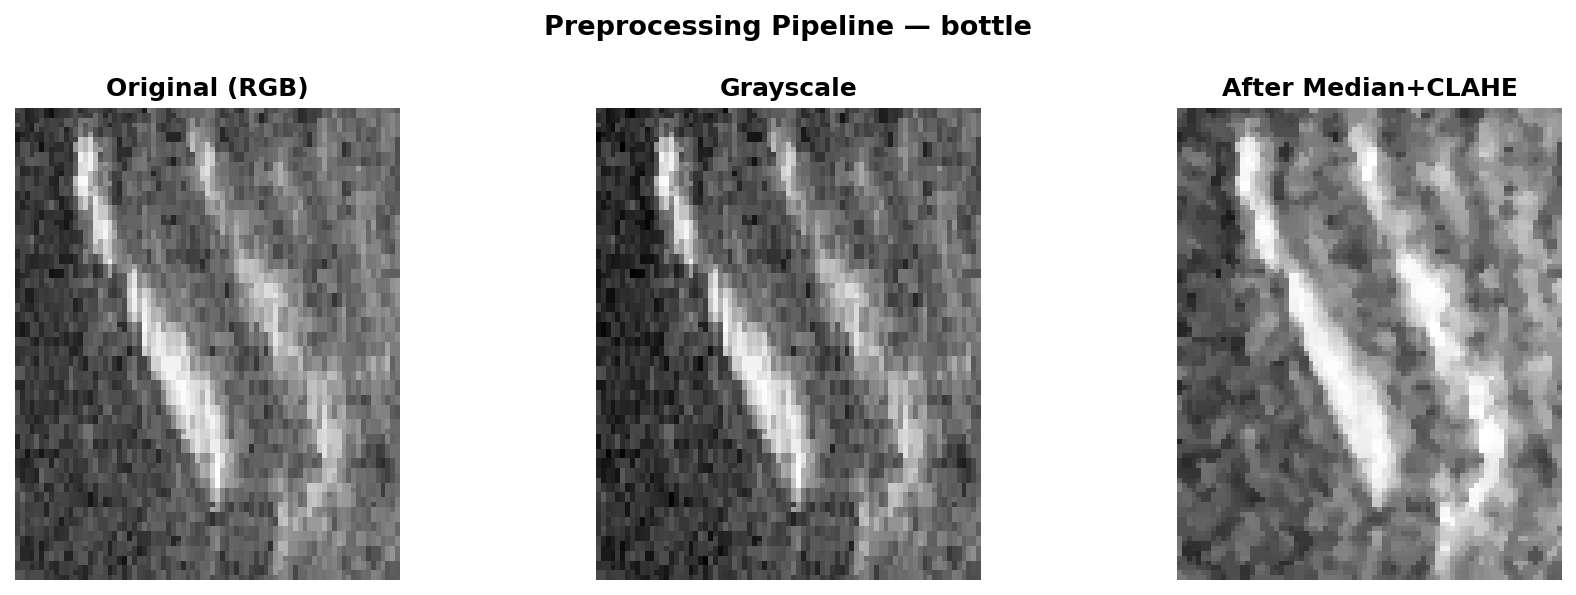
\includegraphics[width=0.92\linewidth]{figures/preprocessing_example.png}
    \caption{Deterministic sonar preprocessing on a \texttt{bottle} crop: RGB input, grayscale conversion, and $3\times 3$ median filtering plus CLAHE ($\text{clipLimit}=2.0$, $8\times 8$ tiles).}
    \label{fig:preproc}
\end{figure}

\subsection{Closed-Set Backbone and MSP Baseline}
\label{sec:msp}

An ImageNet-1K pretrained ResNet-50~\cite{he_2016_resnet} (\texttt{build\_resnet50}) freezes stages \texttt{layer1} and \texttt{layer2} ($1,435,392$ frozen parameters) while updating stages \texttt{layer3}, \texttt{layer4}, the convolutional stem, and a regularized multilayer perceptron (MLP) head ($23,124,806$ trainable out of $24,560,198$ total parameters): $\mathrm{Dropout}(0.3) \to \mathrm{Linear}(2048, 512) \to \mathrm{ReLU} \to \mathrm{Dropout}(0.2) \to \mathrm{Linear}(512, 6)$. Training uses weighted cross-entropy, Adam~\cite{kingma_2015_adam} ($\text{lr}=10^{-4}$, $\text{weight\_decay}=10^{-4}$), \texttt{StepLR} (step size $7$, $\gamma=0.5$), and early stopping on validation accuracy ($\text{patience}=5$, $\text{min\_delta}=0.001$) over $30$ max epochs. Given logits $z(x) \in \mathbb{R}^6$, the MSP baseline~\cite{hendrycks_2017_msp} scores normality as:
\begin{equation}
S_{\mathrm{MSP}}(x) = \max_{k \in \{0,\dots,5\}} \frac{\exp(z_k(x))}{\sum_{j=0}^{5} \exp(z_j(x))}.
\end{equation}

\subsection{2048-D Latent One-Class SVDD Formulations}
\label{sec:svdd}

Stripping the baseline MLP head yields 2048-D GAP vectors $z \in \mathbb{R}^{2048}$ across all 1,233 training and 869 test images. We test three one-class boundaries:
\begin{enumerate}
    \item L2-normalized RBF One-Class SVM~\cite{scholkopf_2001_ocsvm} fitted on unit-norm training embeddings ($\nu = 0.1$, \texttt{gamma='scale'}).
    \item Global Centroid SVDD~\cite{tax_2004_svdd}, scoring negated Euclidean distance to the single global training mean $c$: $S_{\mathrm{global}}(z) = -\|z - c\|_2$.
    \item Nearest Class Centroid SVDD, computing one prototype $c_k$ per known class $k \in \{0,\dots,5\}$ and scoring proximity to the nearest class center:
    \begin{equation}
    S_{\mathrm{nearest}}(z) = -\min_{k \in \{0,\dots,5\}} \|z - c_k\|_2, \quad \hat{y} = \arg\min_{k} \|z - c_k\|_2.
    \end{equation}
\end{enumerate}

\subsection{Hyperspherical Deep Metric Learning (\texttt{EmbeddingNet})}
\label{sec:dml}

Cross-entropy maximizes linear logit separation without constraining intra-class spread or vector norm. Method 3 trains \texttt{EmbeddingNet}, pairing an ImageNet-1K ResNet-50 trunk with a projection head:
\begin{equation}
\mathrm{GAP}(2048) \to \mathrm{Linear}(512) \to \mathrm{BN} \to \mathrm{ReLU} \to \mathrm{Drop}(0.3) \to \mathrm{Linear}(128),
\end{equation}
followed by unit normalization $\hat{e}(x) = e / \|e\|_2 \in \mathbb{S}^{127} \subset \mathbb{R}^{128}$. Because wrapping ResNet children inside \texttt{nn.Sequential} replaces string names with numeric indices, the layer-freezing check evaluates false and all $24,623,808$ parameters fine-tune end-to-end.

Optimization minimizes cosine Triplet Margin Loss~\cite{schroff_2015_facenet,musgrave_2020_pml} ($m = 0.2$) with an online hard triplet miner (\texttt{type\_of\_triplets='hard'}):
\begin{equation}
\mathcal{L}_{\mathrm{triplet}} = \frac{1}{|\mathcal{T}_{\mathrm{hard}}|} \sum_{(a,p,n) \in \mathcal{T}_{\mathrm{hard}}} \max\bigl(0,\, d_{\cos}(\hat{e}_a, \hat{e}_n) - d_{\cos}(\hat{e}_a, \hat{e}_p) + 0.2\bigr),
\end{equation}
where $d_{\cos}(u, v) = u^\top v$ for unit vectors. We use Adam ($\text{lr}=10^{-4}$, $\text{weight\_decay}=10^{-4}$), \texttt{StepLR} ($7$, $0.5$), and early stopping on validation triplet loss ($\text{patience}=5$, $\text{min\_delta}=0.001$) over $30$ max epochs. Six class centroids $c_k^{\mathrm{metric}} \in \mathbb{R}^{128}$ give the inference score $S_{\mathrm{DML}}(x) = -\min_k \|\hat{e}(x) - c_k^{\mathrm{metric}}\|_2$.

\subsection{Evaluation Protocol}
\label{sec:eval}

Known test samples ($271$) have binary label $1$ and unknown test samples ($598$) have label $0$. We report threshold-independent Area Under the ROC Curve ($\mathrm{AUROC} \uparrow$) and Average Precision ($\mathrm{AP} \uparrow$, critical when unknowns outnumber knowns). Operating points $\tau^*$ maximize Youden's $J = \mathrm{TPR}(\tau) - \mathrm{FPR}(\tau)$~\cite{youden_1950_index}, giving True Positive Rate ($\mathrm{TPR} \uparrow$), False Positive Rate ($\mathrm{FPR} \downarrow$), and Unknown Detection Rate ($\mathrm{UDR} = 1 - \mathrm{FPR} \uparrow$).

\section{Experiments, Results, and Failure Analysis}
\label{sec:results}

\subsection{Closed-Set Classification Verification}
\label{sec:closed}

Both backbones establish strong closed-set classification before open-set rejection is applied. The ResNet-50 baseline converged within $12$ epochs at $99.2\%$ best validation accuracy and reached $99.26\%$ overall test accuracy ($269 / 271$ correct) across the six known categories (Table~\ref{tab:closed}). Four classes (\texttt{can}, \texttt{tire}, \texttt{drink-carton}, \texttt{hook}) had zero test errors; two test samples were confused (\texttt{bottle} predicted as \texttt{can}, \texttt{propeller} as \texttt{tire}), giving a macro-average F1 score of $0.9918$. In the $128$-D embedding space, nearest-centroid classification on the same $271$ known test samples reached $100.00\%$ accuracy (\texttt{closed\_acc} $= 1.0$).

\begin{table}[!htbp]
\centering
\caption{Closed-Set Test Performance on $271$ Known Samples}
\label{tab:closed}
\footnotesize
\setlength{\tabcolsep}{3.5pt}
\begin{tabular}{@{}lcccc@{}}
\toprule
Known Class & Precision & Recall & F1-Score & Support \\
\midrule
\texttt{bottle}       & 1.0000 & 0.9853 & 0.9926 & 68 \\
\texttt{can}          & 0.9825 & 1.0000 & 0.9912 & 56 \\
\texttt{tire}         & 0.9808 & 1.0000 & 0.9903 & 51 \\
\texttt{drink-carton} & 1.0000 & 1.0000 & 1.0000 & 53 \\
\texttt{hook}         & 1.0000 & 1.0000 & 1.0000 & 21 \\
\texttt{propeller}    & 1.0000 & 0.9545 & 0.9767 & 22 \\
\midrule
Weighted Avg (269/271) & 0.9928 & 0.9926 & 0.9926 & 271 \\
Macro Avg              & 0.9939 & 0.9900 & 0.9918 & 271 \\
DML Nearest Cent.      & \multicolumn{3}{c}{Closed Acc: $100.0\%$} & 271 \\
\bottomrule
\end{tabular}
\end{table}

\subsection{Unified Open-Set Recognition Benchmark}
\label{sec:unified}

Table~\ref{tab:osr_bench} and Fig.~\ref{fig:all_comp} compare all five configurations across the $869$-image open-set test set ($271$ known, $598$ unknown). Deep Metric Learning leads every metric: $0.9603$ $\mathrm{AUROC}$, $0.9235$ $\mathrm{AP}$, $0.9077$ $\mathrm{TPR}$, $0.0987$ $\mathrm{FPR}$, and $0.9013$ $\mathrm{UDR}$ at Youden threshold $\tau^* = -0.2378$. Compared against MSP ($0.9069$ $\mathrm{AUROC}$, $0.7747$ $\mathrm{AP}$), DML cuts false unknown acceptances from $87$ to $59$ and raises accepted knowns from $236$ to $246$. Nearest Class Centroid SVDD ranks second overall ($0.9175$ $\mathrm{AUROC}$, $0.8568$ $\mathrm{AP}$, $0.8595$ $\mathrm{UDR}$) without metric retraining.

\begin{table*}[!t]
\centering
\caption{Unified Open-Set Recognition Benchmark on $869$ Combined MD-FLS Water-Tank Test Images ($271$ Known, $598$ Unknown)}
\label{tab:osr_bench}
\footnotesize
\setlength{\tabcolsep}{4pt}
\begin{tabular}{@{}llccccccc@{}}
\toprule
Method / Variant & Feature Space & $\mathrm{AUROC} \uparrow$ & $\mathrm{AP} \uparrow$ & $\mathrm{TPR} \uparrow$ & $\mathrm{FPR} \downarrow$ & $\mathrm{UDR} \uparrow$ & Threshold $\tau^*$ & TP / FN / TN / FP \\
\midrule
MSP Threshold          & 6-D Softmax          & 0.9069 & 0.7747 & 0.8708 & 0.1455 & 0.8545 & 0.9980   & 236 / 35 / 511 / 87 \\
SVDD: OC-SVM (RBF)     & 2048-D L2-norm       & 0.6982 & 0.3943 & 0.9926 & 0.5100 & 0.4900 & --       & -- \\
SVDD: Global Centroid  & 2048-D Raw GAP       & 0.2371 & 0.2064 & 0.9815 & 0.9298 & 0.0702 & --       & -- \\
SVDD: Nearest Centroid & 2048-D Raw GAP       & 0.9175 & 0.8568 & 0.8856 & 0.1405 & 0.8595 & $-13.8392$ & 240 / 31 / 514 / 84 \\
Deep Metric Learning   & 128-D Unit Sphere    & \textbf{0.9603} & \textbf{0.9235} & \textbf{0.9077} & \textbf{0.0987} & \textbf{0.9013} & $-0.2378$ & \textbf{246 / 25 / 539 / 59} \\
\bottomrule
\end{tabular}
\end{table*}

\begin{figure*}[!t]
    \centering
    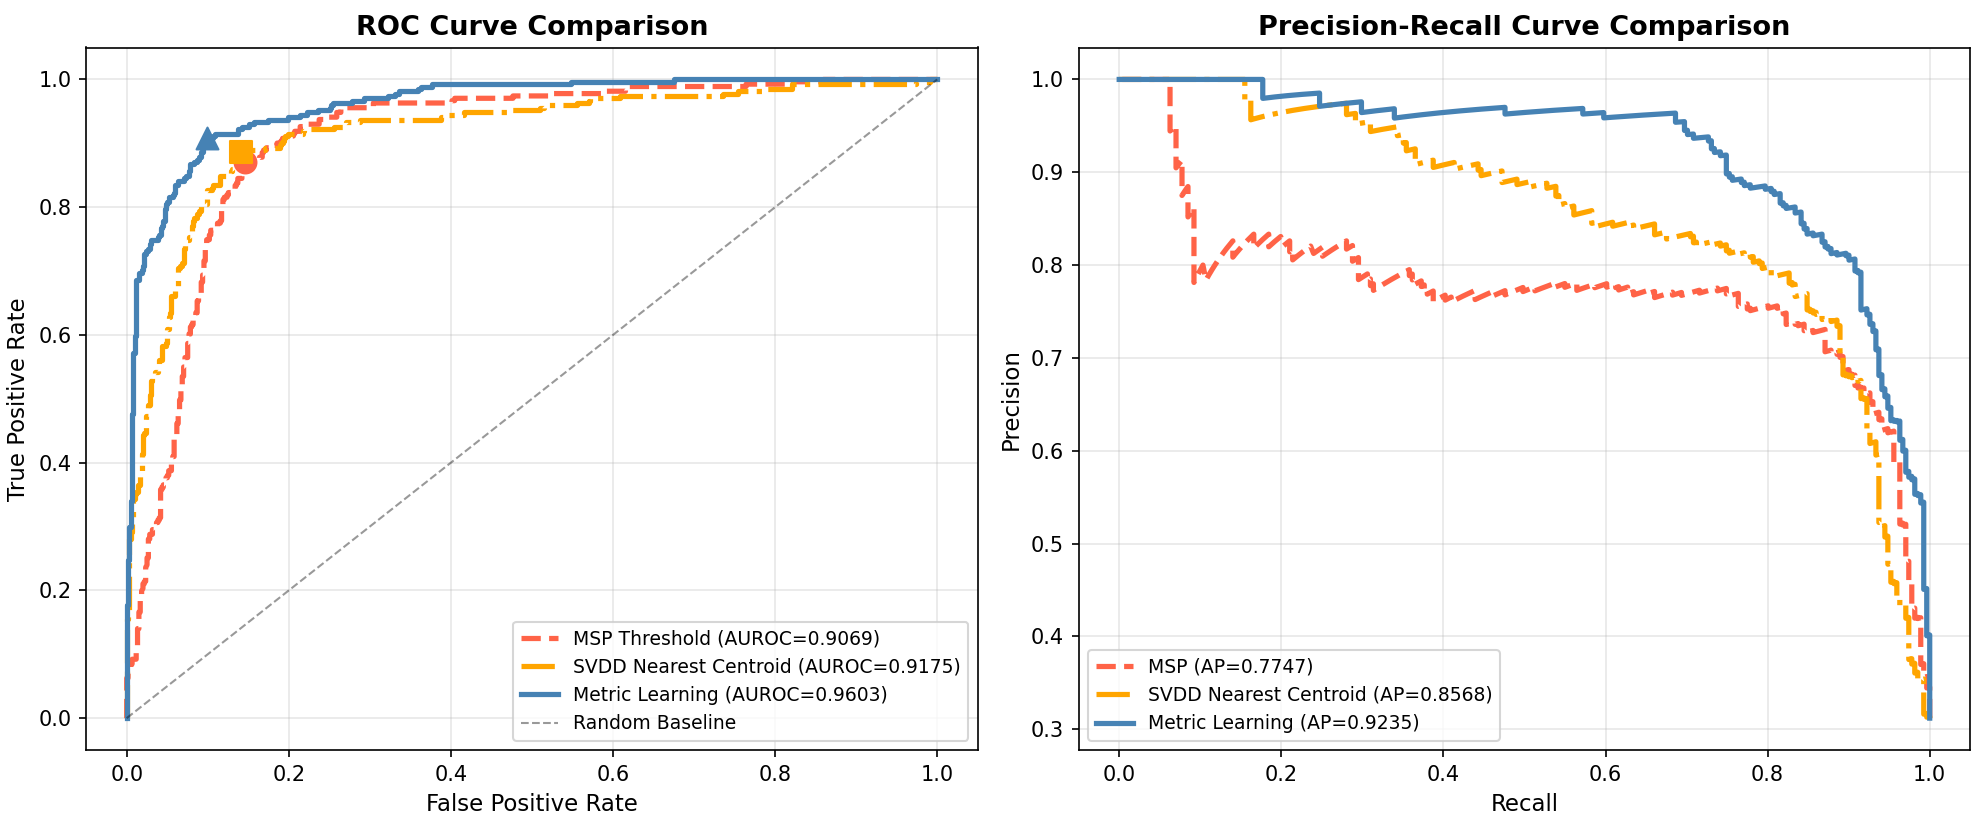
\includegraphics[width=0.68\textwidth]{figures/osr_roc_pr_comparison.png}
    \caption{Cross-method ROC (left) and Precision-Recall (right) curves on the $869$-image test set. Deep Metric Learning improves $\mathrm{AP}$ from $0.7747$ (MSP) and $0.8568$ (SVDD Nearest) to $0.9235$ while leading $\mathrm{AUROC}$ ($0.9603$).}
    \label{fig:all_comp}
\end{figure*}

\begin{figure*}[!t]
    \centering
    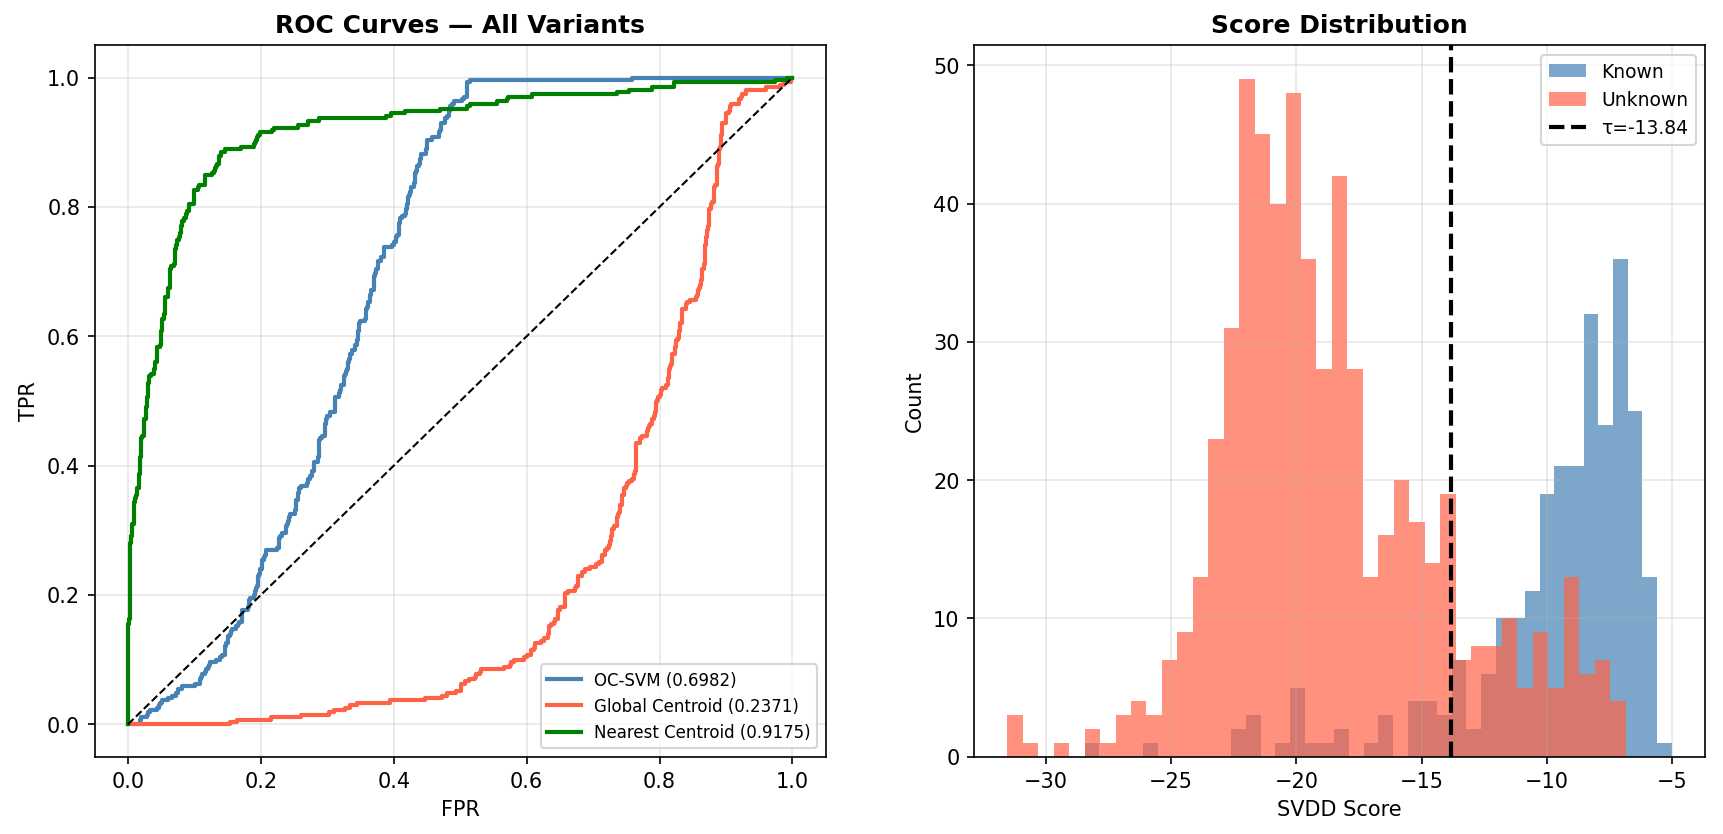
\includegraphics[width=0.64\textwidth]{figures/svdd_failure_panels.png}
    \caption{SVDD failure diagnosis on 2048-D GAP features. Left: Global Centroid collapses below random chance ($\mathrm{AUROC}=0.2371$), L2 OC-SVM partially recovers ($0.6982$), and Nearest Centroid reaches $0.9175$. Right: Nearest Centroid score distribution separating known and unknown test samples around $\tau^*=-13.84$.}
    \label{fig:svdd_dash}
\end{figure*}

\subsection{Failure Analysis I: Global Centroid SVDD Collapse}
\label{sec:svdd_collapse}

Comparing the three SVDD variants exposes a geometric collapse in raw GAP space (Fig.~\ref{fig:svdd_dash}, left). Enclosing all $1,233$ known training embeddings around one Global Centroid scores $\mathrm{AUROC} = 0.2371$, $\mathrm{AP} = 0.2064$, $\mathrm{UDR} = 0.0702$, and $\mathrm{FPR} = 0.9298$, inverting normal-versus-unknown ordering well below random chance. While deep one-class learners risk hypersphere collapse~\cite{chong_2020_ijcnn}, supervised cross-entropy creates an inverse mismatch for post-hoc single-center SVDD: known classes occupy separated high-norm radial lobes in $\mathbb{R}^{2048}$, placing the arithmetic mean $c$ in an underpopulated central region. Unknown sonar patches lacking strong known-class filter responses fall closer to $c$ than known objects sitting out on class lobes.

L2 normalization with an RBF One-Class SVM ($\nu=0.1$) removes norm bias ($\mathrm{AUROC} = 0.6982$, $\mathrm{UDR} = 0.4900$), yet still suffers $51.00\%$ false unknown acceptance because a single boundary bridges inter-class voids. Switching to six per-class centroids ($S_{\mathrm{nearest}}$) wraps each lobe locally, raising $\mathrm{AUROC}$ from $0.2371$ to $0.9175$ and lowering $\mathrm{FPR}$ to $0.1405$ (Fig.~\ref{fig:svdd_dash}, right).

\subsection{Failure Analysis II: Softmax Confidence Compression}
\label{sec:msp_failure}

While MSP ranks samples at $0.9069$ $\mathrm{AUROC}$, its $\mathrm{AP}$ stops at $0.7747$ (below $0.8568$ for SVDD Nearest and $0.9235$ for DML). Unbounded linear logit sectors saturate posteriors near unity~\cite{bendale_2016_openmax}: Fig.~\ref{fig:msp_dist} shows nearly all $271$ known images compressed near $1.0$ while a large mode of unknown samples piles into the top confidence bin. Youden optimization therefore selects $\tau^* = 0.9980$, leaving virtually zero threshold slack before admitting unfamiliar debris.

\begin{figure}[!htbp]
    \centering
    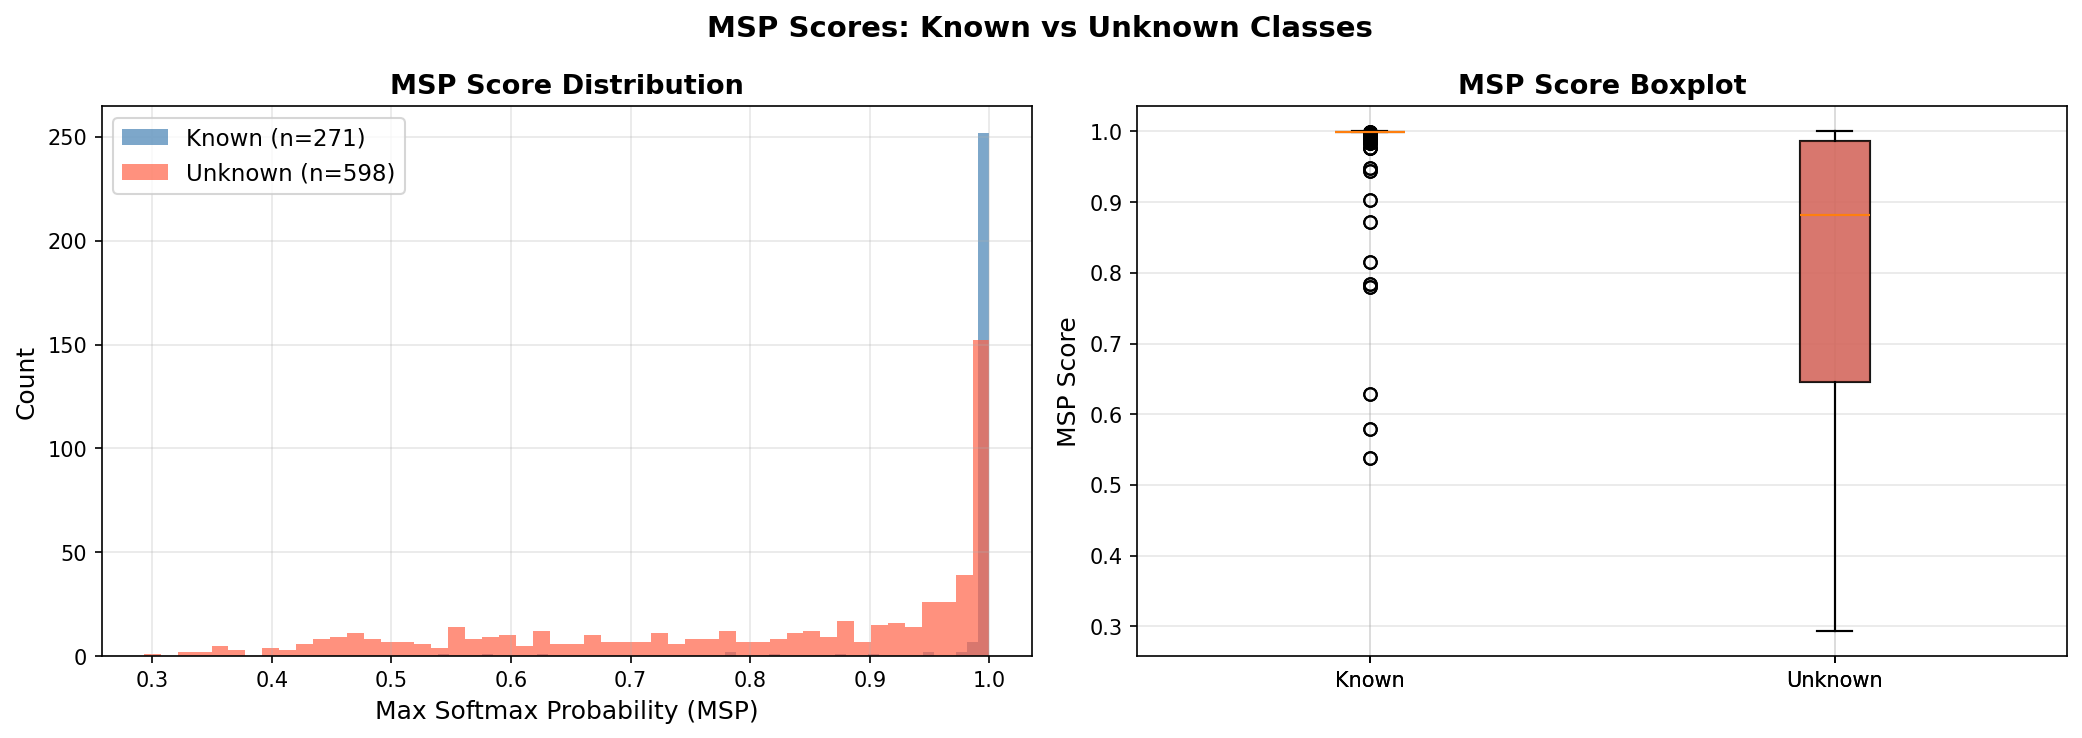
\includegraphics[width=0.92\linewidth]{figures/msp_distributions.png}
    \caption{MSP confidence distribution and boxplot ($271$ known vs. $598$ unknown). Dense unknown accumulation near unity pushes $\tau^*$ to $0.9980$ and limits Average Precision to $0.7747$.}
    \label{fig:msp_dist}
\end{figure}

\begin{figure*}[!t]
    \centering
    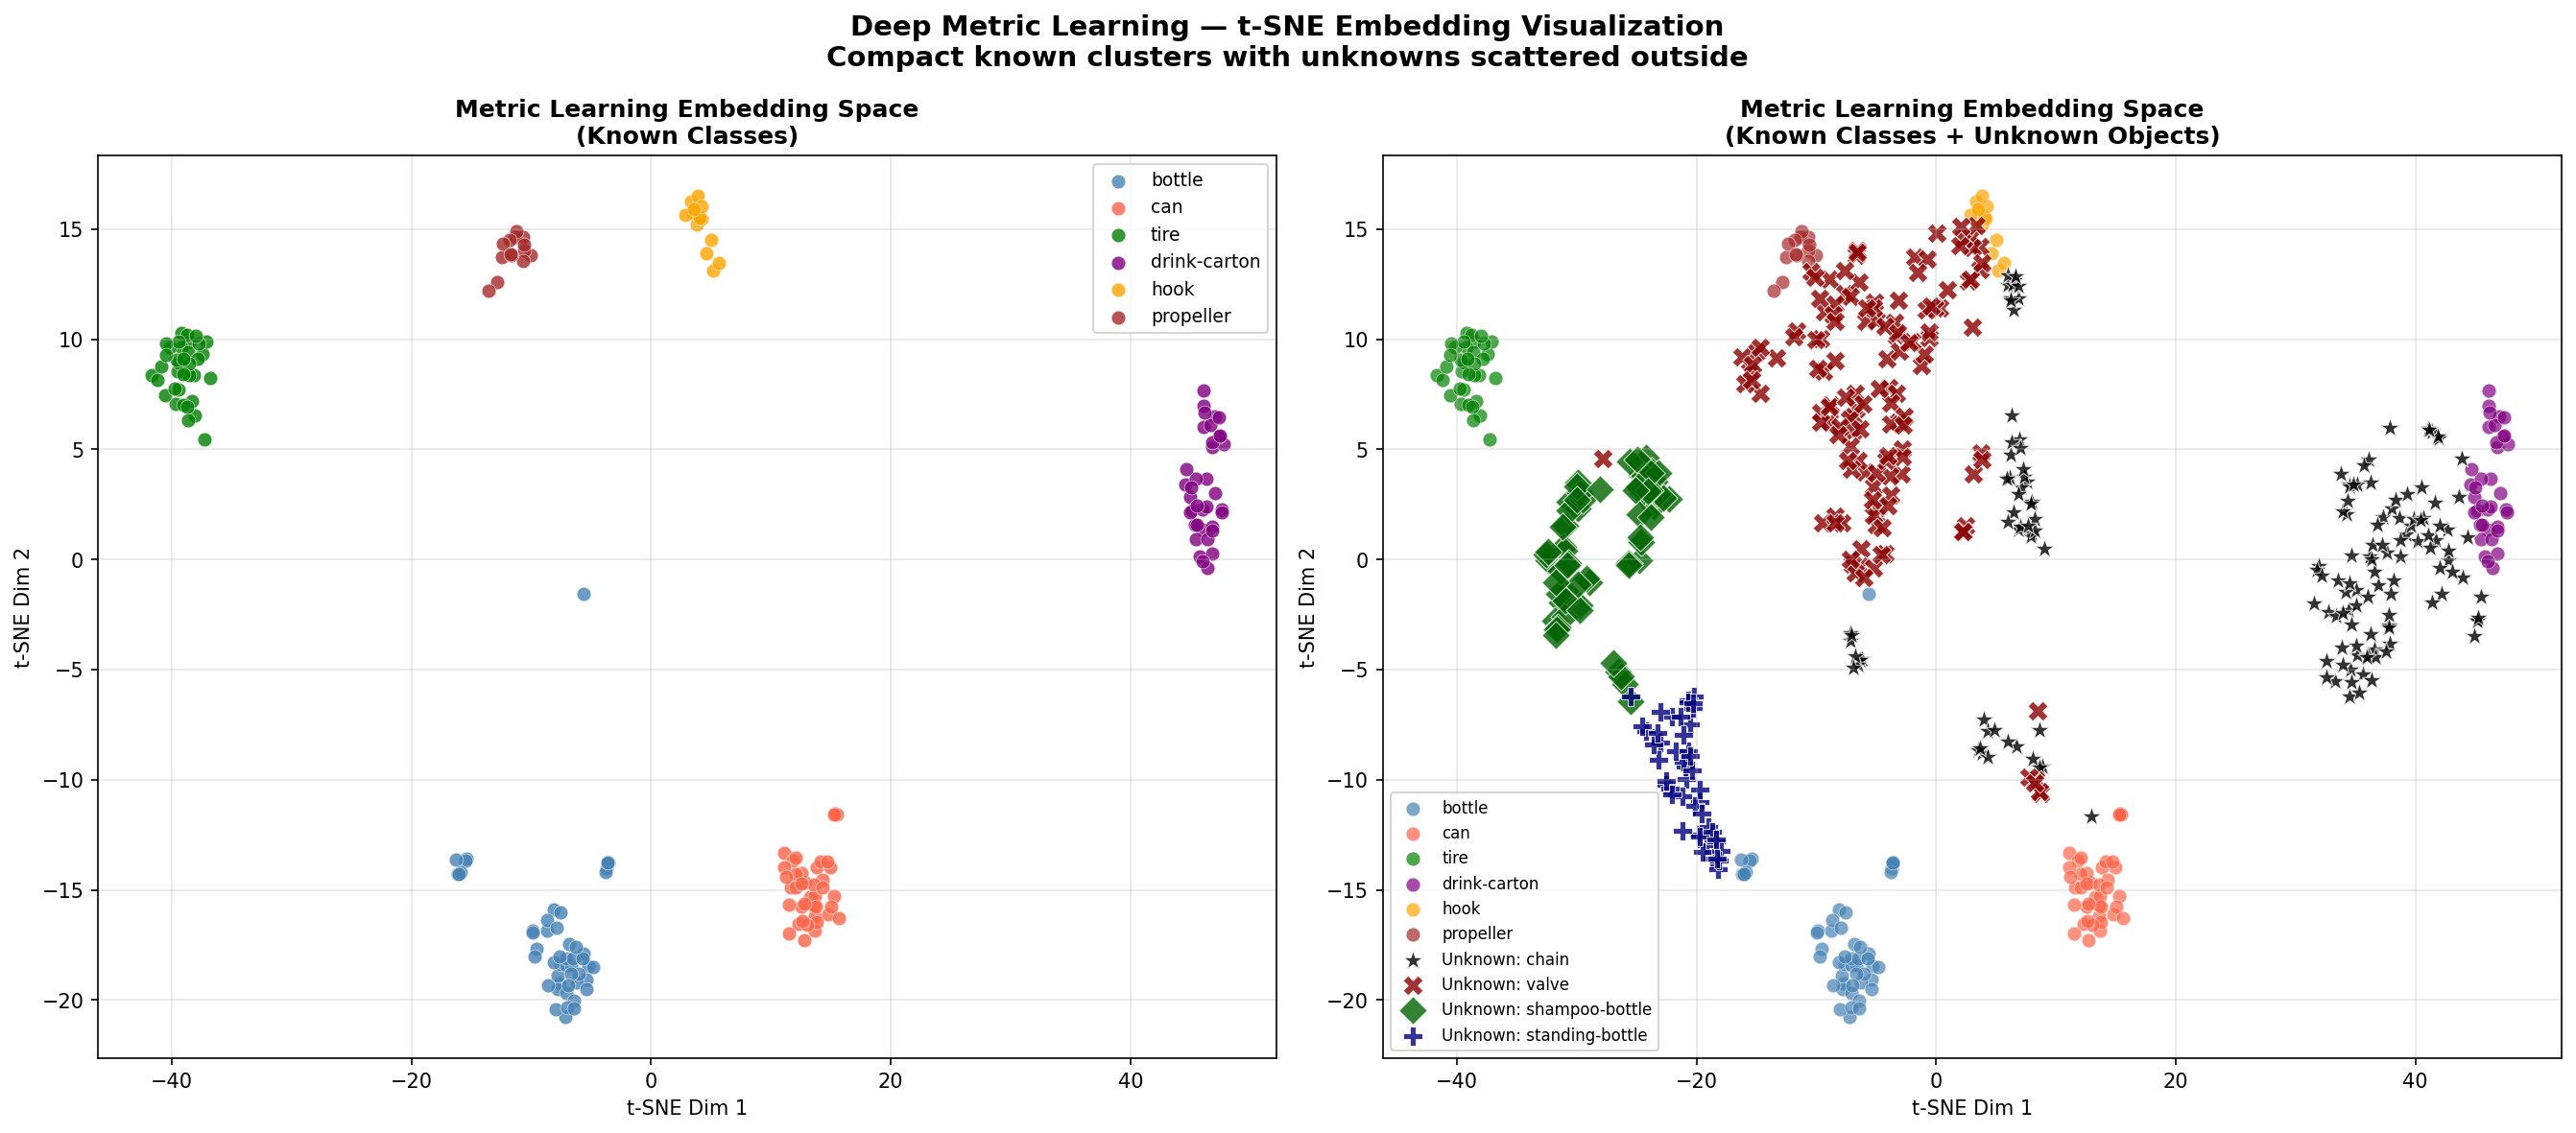
\includegraphics[width=0.70\textwidth]{figures/dml_tsne_visualization.png}
    \caption{Two-dimensional t-SNE projection of test embeddings from the $128$-D L2-normalized \texttt{EmbeddingNet} space. Left: known classes form tight isolated clusters. Right: unknown targets occupy peripheral and interstitial space, separating \texttt{shampoo-bottle} and \texttt{standing-bottle} cleanly outside known clusters.}
    \label{fig:tsne}
\end{figure*}

\subsection{Per-Unknown-Class Breakdown and Embedding Geometry}
\label{sec:perclass}

Table~\ref{tab:per_unknown} breaks down unknown rejection across all four withheld classes ($598$ images). At Youden thresholds ($\tau^* = 0.9980$, $-13.8392$, and $-0.2378$), all three methods reject $100.00\%$ of \texttt{shampoo-bottle} ($99$ of $99$) and \texttt{standing-bottle} ($65$ of $65$). For MSP, however, that $100.00\%$ rejection relies on pushing $\tau^*$ up to $0.9980$ (losing $35$ known targets), whereas distance scoring separates elongated container crops directly in latent space. On \texttt{valve} ($208$ images), MSP rejects $94.71\%$ ($197$), DML rejects $92.79\%$ ($193$), and Nearest Centroid rejects $91.35\%$ ($190$).

The hardest category across all methods is \texttt{chain} ($226$ images), whose segmented metallic links resemble \texttt{hook} and \texttt{bottle} contours in single sonar views. Rejection improves from $66.37\%$ ($150$) in MSP and $70.80\%$ ($160$) in SVDD Nearest Centroid to $80.53\%$ ($182$) in DML. Fig.~\ref{fig:tsne} visualizes test embeddings from the $128$-D unit hypersphere via t-SNE (seed $42$): the six known classes form compact clusters (left), \texttt{shampoo-bottle} and \texttt{standing-bottle} separate cleanly outside \texttt{bottle} and \texttt{tire}, \texttt{valve} spans upper-central interstitial space, and \texttt{chain} clusters beside \texttt{drink-carton} with residual points near \texttt{hook} and \texttt{can}.

\begin{table}[!htbp]
\centering
\caption{Per-Unknown-Class Rejection Rate ($\%$ and Counts)}
\label{tab:per_unknown}
\footnotesize
\setlength{\tabcolsep}{3pt}
\begin{tabular}{@{}lcccc@{}}
\toprule
Unknown Class & Total & MSP ($\tau^*=0.9980$) & SVDD Nearest & DML \\
\midrule
\texttt{chain}           & 226 & 66.37\% (150) & 70.80\% (160) & \textbf{80.53\% (182)} \\
\texttt{valve}           & 208 & \textbf{94.71\% (197)} & 91.35\% (190) & 92.79\% (193) \\
\texttt{shampoo-bottle}  & 99  & 100.00\% (99) & 100.00\% (99) & 100.00\% (99) \\
\texttt{standing-bottle} & 65  & 100.00\% (65) & 100.00\% (65) & 100.00\% (65) \\
\midrule
Overall UDR              & 598 & 85.45\% (511) & 85.95\% (514) & \textbf{90.13\% (539)} \\
\bottomrule
\end{tabular}
\end{table}

\section{Limitations and Future Work}
\label{sec:limits}

Four scope boundaries qualify these results and define next experiments:
\begin{enumerate}
    \item Single seed and threshold calibration: all splits and training runs use deterministic seed $42$ without multi-seed variance bands. Operating thresholds $\tau^*$ maximize Youden's $J$ on the test ROC curve; production deployment requires calibrating $\tau$ on a held-out proxy-outlier validation fold.
    \item Backbone trainability difference: wrapping ResNet children inside \texttt{nn.Sequential} keeps all $24,623,808$ parameters trainable in \texttt{EmbeddingNet}, whereas \texttt{build\_resnet50} freezes \texttt{layer1} and \texttt{layer2} ($23,124,806$ trainable). DML's gain reflects joint backbone adaptation combined with cosine triplet supervision.
    \item Water-tank domain and unexecuted turntable testing: evaluation uses cropped water-tank FLS imagery only. Open-ocean deployment adds multipath reverberation and range attenuation; cross-domain testing on the 18-class MD-FLS turntable subset~\cite{valdenegro_2025_datasets} and direct benchmarking against EVT logit methods~\cite{bendale_2016_openmax,li_2026_copenmax} remain future work.
    \item Single-ping ambiguity: 2D FLS projection drops elevation structure, leaving $44$ of $226$ \texttt{chain} patches misaccepted by DML from single frames. Multi-frame ping fusion across AUV trajectories should reduce this geometric overlap.
\end{enumerate}

\section{Conclusion}
\label{sec:conclusion}

We compared Softmax MSP, three 2048-D SVDD boundaries, and hyperspherical Deep Metric Learning on 2,364 MD-FLS water-tank images across six known and four unseen marine debris categories. Although closed-set ResNet-50 achieves 99.26\% test accuracy, MSP scores pile up near 0.9980 (0.7747 AP, 0.9069 AUROC) and Global Centroid SVDD collapses to 0.2371 AUROC because cross-entropy separates known classes onto outer radial lobes. Switching to Nearest Class Centroid SVDD lifts performance to 0.9175 AUROC (0.8568 AP), and end-to-end cosine Triplet Margin Learning onto the 128-D unit hypersphere leads all five metrics: 0.9603 AUROC, 0.9235 AP, 0.9013 UDR, 0.0987 FPR, 0.9077 TPR, 100.0\% closed-set known accuracy, and 80.53\% detection on the hardest unknown class (\texttt{chain}). Multi-seed proxy-outlier threshold calibration and cross-domain MD-FLS turntable evaluation are the immediate next steps toward field AUV deployment.

\section*{Acknowledgment}
The authors thank the creators of the public Marine Debris Forward-Looking Sonar (MD-FLS) datasets for releasing open underwater acoustic benchmarks and acknowledge Kaggle GPU compute resources used for model training and evaluation.

\bibliographystyle{IEEEtran}
\bibliography{references}

\end{document}
